\documentclass[xetex,mathserif,serif]{beamer}
\usepackage{polyglossia}
\setdefaultlanguage[babelshorthands=true]{russian}
\usepackage{minted}
\usemintedstyle{borland}

\usetheme{SPbGU}

\setmainfont{FreeSans}

\def\settt#1{\expandafter#1
  [Path=./fonts/,Scale=0.8,
   BoldFont=JetBrainsMonoNL-Bold.ttf,
   ItalicFont=JetBrainsMonoNL-Italic.ttf,
   BoldItalicFont=JetBrainsMonoNL-BoldItalic.ttf
  ]{JetBrainsMonoNL-Regular.ttf}
}
\settt{\setmonofont}
\settt{\newfontfamily{\cyrillicfonttt}}

\definecolor{links}{HTML}{2A1B81}
\hypersetup{colorlinks,linkcolor=,urlcolor=links}

\title{Лекция <<Парадигмы программирования>>}
\author[Юрий Литвинов]{Юрий Литвинов \newline \textcolor{gray}{\small\texttt{yurii.litvinov@gmail.com}}}
\date{}

\begin{document}
{
\setbeamertemplate{footline}{}
\begin{frame}
  
\includegraphics[width=1.4cm]{pictures/SPbGU_Logo.png}
\vspace{-35pt}
\hspace{-10pt}
\begin{center}
   \begin{tabular}{c}
        \scriptsize{Санкт-Петербургский государственный университет} \\
        \scriptsize{Кафедра системного программирования}
    \end{tabular}
\titlepage
\end{center}

\btVFill

\begin{center}
  \vspace{5pt}
  \scriptsize{Санкт-Петербург\\
                 2020}
  \end{center}

\end{frame}
}

    \section{Введение}

    \begin{frame}
        \frametitle{О чём пойдёт речь}
        \begin{itemize}
            \item Опыт кафедры системного программирования СПбГУ в подготовке образовательного контента
            \item Пример (сокращённый) лекции для студентов 1-го курса бакалавриата <<Технологии программирования>>
            \item Обсуждение места лекции в курсе и программе в целом, опыт прочтения
            \item Инструменты для разработки материалов
        \end{itemize}
    \end{frame}

    \section{Лекция}

    \begin{frame}
        \frametitle{Математические модели вычислений}
        \begin{itemize}
            \item Что можно посчитать имея вычислительную машину неограниченной мощности?
            \item Формальные модели вычислений:
            \begin{itemize}
                \item Машина Тьюринга
                \item $\lambda$-исчисление Чёрча
                \item Нормальные алгорифмы Маркова
            \end{itemize}
            \item Тезис Чёрча: <<Любая функция, которая может быть вычислена физическим устройством, может быть вычислена машиной Тьюринга>>
        \end{itemize}
    \end{frame}

    \begin{frame}
        \frametitle{Машина Тьюринга}
        \begin{columns}
            \begin{column}{0.6\textwidth}
                \begin{itemize}
                    \item Формально,
                        $$M = (Q, \Gamma, b, \Sigma, \delta, q_0, F)$$
                        $$\delta : (Q / F) × \Gamma \rightarrow Q × \Gamma × \{L, R\}$$
                    \item Неформально:
                    \begin{itemize}
                        \item Бесконечная лента с символами из $\Sigma$ и $b$
                        \item Считывающая головка
                        \item Внутренняя память $Q$
                        \item Таблица переходов $\delta$, которая по текущему состоянию из $Q$ и текущему символу на ленте из $\Gamma$ говорит машине, что делать:
                        \begin{itemize}
                            \item перейти в состояние
                            \item записать символ на ленту
                            \item сместиться влево/вправо
                        \end{itemize}
                    \end{itemize}
                \end{itemize}
            \end{column}
            \begin{column}{0.4\textwidth}
                \begin{center}
                    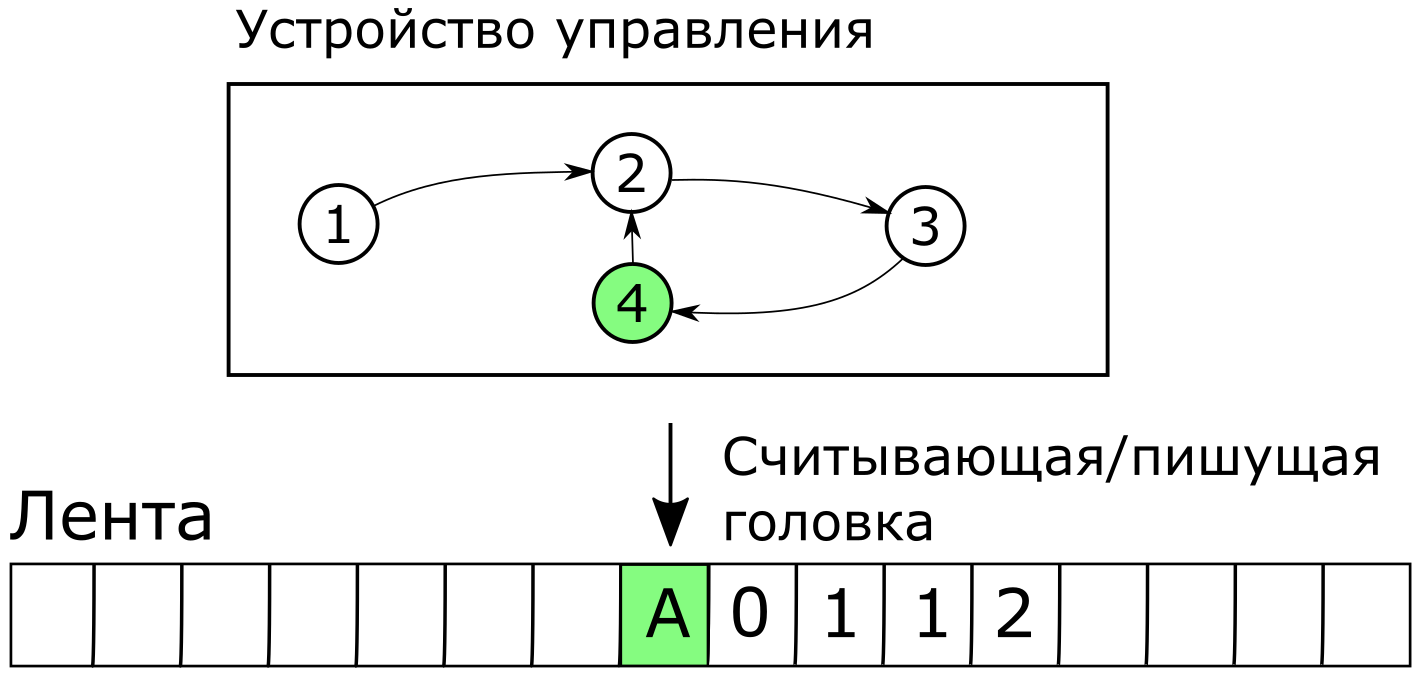
\includegraphics[width=\textwidth]{turingMachine.png}
                \end{center}
            \end{column}
        \end{columns}
    \end{frame}

    \begin{frame}
        \frametitle{Архитектура фон Неймана}
        \begin{columns}
            \begin{column}{0.6\textwidth}
                \begin{itemize}
                    \item Принцип последовательного программного управления
                    \item Принцип однородности памяти
                    \item Принцип адресуемости памяти
                    \item Принцип двоичного кодирования
                    \item Принцип жесткости архитектуры
                \end{itemize}
            \end{column}
            \begin{column}{0.4\textwidth}
                \begin{center}
                    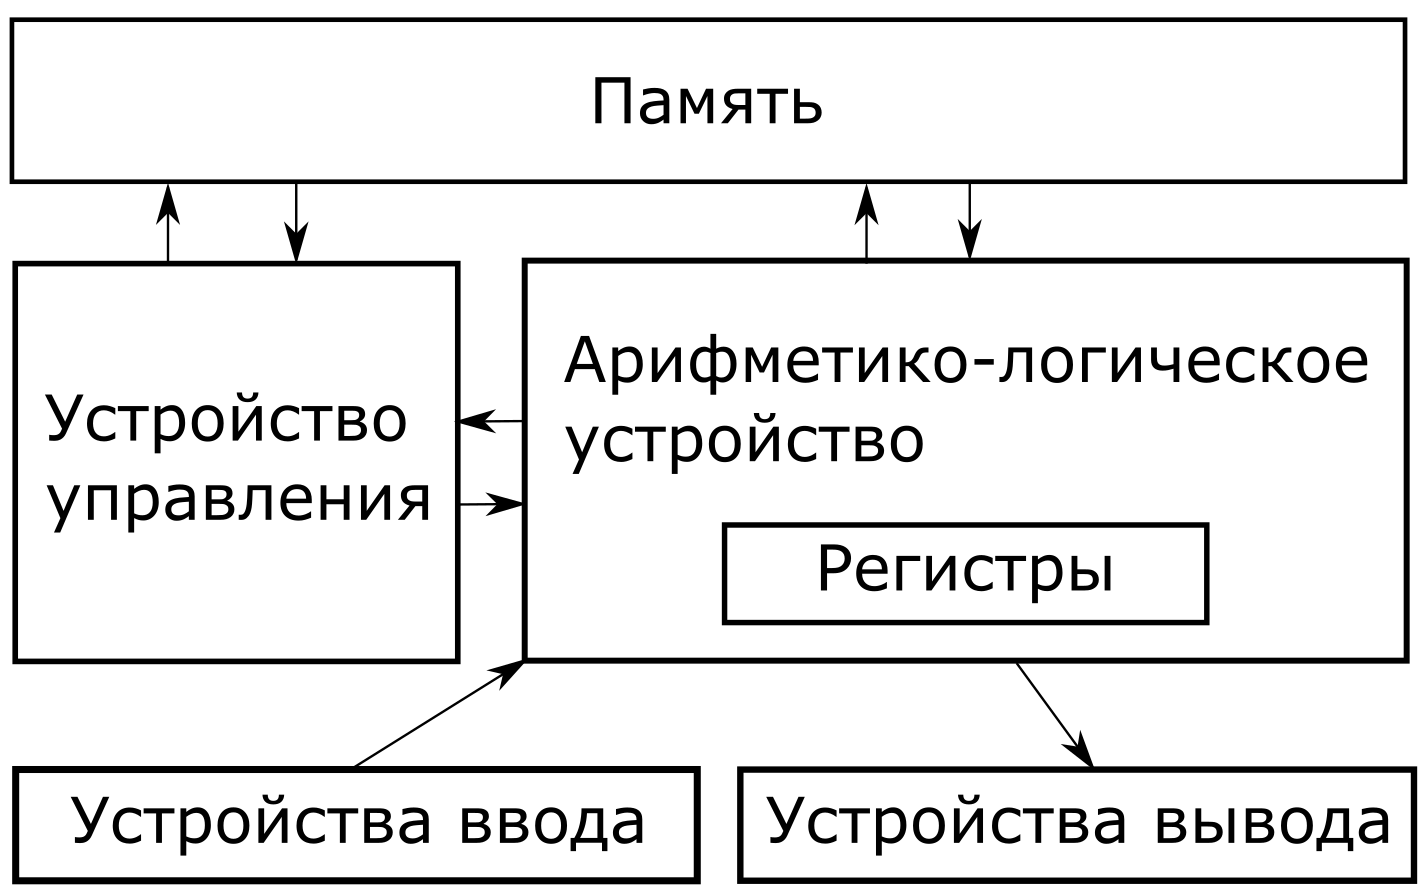
\includegraphics[width=\textwidth]{vonNeumannArchitecture.png}
                \end{center}
            \end{column}
        \end{columns}
    \end{frame}

    \begin{frame}
        \frametitle{Структурное программирование}
        \begin{itemize}
            \item Пришло на смену неструктурированному программированию в начале 70-х
            \begin{itemize}
                \item FORTRAN --- 1957 год, язык высокого уровня, но не структурный
            \end{itemize}
            \item Любая программа может быть представлена как комбинация
            \begin{itemize}
                \item последовательно исполняемых операторов
                \item ветвлений
                \item итераций
            \end{itemize}
            \item Статья Дейкстры <<Go To Statement Considered Harmful>> (1968г)
        \end{itemize}
    \end{frame}

    \begin{frame}
        \frametitle{Языки-представители}
        \begin{itemize}
            \item Алгол
            \item Паскаль
            \item C
            \item Модула-2
            \item Ада
        \end{itemize}
    \end{frame}

    \begin{frame}[fragile]
        \frametitle{Подробнее: Ада}
        \begin{itemize}
            \item Разработан в начале 80-х по заказу минобороны США
            \item Особенности:
            \begin{itemize}
                \item Строгая типизация
                \item Минимум автоматических преобразований типов
                \item Встроенная поддержка параллелизма
            \end{itemize}
            \item Реализация: GNAT (\url{https://www.adacore.com/community})
        \end{itemize}
        \begin{minted}{ada}
    with Ada.Text_IO;
    use Ada.Text_IO;

    procedure Main is
    begin
        Put_Line ("Hello World");
    end Main;
        \end{minted}
    \end{frame}

    \begin{frame}[fragile]
        \frametitle{Ада, модульная система}
        \begin{minted}{ada}
package types is
    type Type_1 is private;
    type Type_2 is private;
    type Type_3 is private;
    procedure P(X: Type_1);
    ...
private
    procedure Q(Y: Type_1);
    type Type_1 is new Integer range 1 .. 1000;
    type Type_2 is array (Integer range 1 .. 1000) of Integer;
    type Type_3 is record
        A, B: Integer;
    end record;
end Types;
        \end{minted}
    \end{frame}

    \begin{frame}[fragile]
        \frametitle{Ада, многопоточность и рандеву}
        \begin{small}
            \begin{minted}{ada}
with Ada.Text_IO; use Ada.Text_IO;

procedure Main is
    task After is
        entry Go(Text: String);
    end After;

    task body After is
    begin
        accept Go(Text: String) do
            Put_Line("After: " & Text);
        end Go;
    end After;
begin
    Put_Line("Before");
    After.Go("Main");
end;
            \end{minted}
        \end{small}
    \end{frame}

    \begin{frame}[fragile]
        \frametitle{Ада, ограничения и контракты}
        \begin{minted}{ada}
type Not_Null is new Integer
    with Dynamic_Predicate => Not_Null /= 0;

type Even is new Integer
    with Dynamic_Predicate => Even mod 2 = 0;

function Divide (Left, Right : Float) return Float
    with Pre => Right /= 0.0,
         Post => Divide'Result * Right < Left + 0.0001
                 and then Divide'Result * Right > Left - 0.0001;
        \end{minted}
    \end{frame}

    \begin{frame}
        \frametitle{Объектно-ориентированное программирование}
        \begin{itemize}
            \item Первый ОО-язык --- Симула-67, были и более ранние разработки
            \item Популярной методология стала только в середине 90-х
            \item Развитие связано с широким распространением графических интерфейсов и компьютерных игр
        \end{itemize}
    \end{frame}

    \begin{frame}
        \frametitle{Основные концепции}
        \begin{itemize}
            \item Программа представляет собой набор объектов
            \item Объекты взаимодействуют путём посылки сообщений по строго определённым интерфейсам
            \item Объекты имеют своё состояние и поведение
            \item Каждый объект является экземпляром некоего класса
        \end{itemize}
    \end{frame}

    \begin{frame}
        \frametitle{Основные концепции (инкапсуляция)}
        \begin{itemize}
            \item Инкапсуляция --- сокрытие реализации от пользователя
            \item Пользователь может взаимодействовать с объектом только через интерфейс
            \item Позволяет менять реализацию объекта, не модифицируя код, который этот объект использует
        \end{itemize}
    \end{frame}

    \begin{frame}
        \frametitle{Основные концепции (наследование)}
        \begin{itemize}
            \item Наследование позволяет описать новый класс на основе существующего, наследуя его свойства и функциональность
            \item Наследование --- отношение <<является>> между классами, с классом-наследником можно обращаться так же, как с классом-предком
            \begin{itemize}
                \item Принцип подстановки Барбары Лисков
            \end{itemize}
        \end{itemize}
    \end{frame}

    \begin{frame}
        \frametitle{Основные концепции (полиморфизм)}
        \begin{itemize}
            \item Полиморфизм --- классы-потомки могут изменять реализацию методов класса-предка, сохраняя их сигнатуру
            \item Клиенты могут работать с объектами класса-родителя, но вызываться будут методы класса-потомка (позднее связывание)
        \end{itemize}
    \end{frame}

    \begin{frame}[fragile]
        \frametitle{Пример кода}
        \begin{minted}{cpp}
class Animal
{
    public:
        Animal(const string& name) { 
            this.name = name; 
        }

        void rename(const string &newName) { 
            name = newName; 
        }

        virtual string talk() = 0;

    private:
        string name;
};
        \end{minted}
    \end{frame}

    \begin{frame}[fragile]
        \frametitle{Пример кода (2)}
        \begin{minted}{cpp}
class Cat : public Animal
{
    public:
        Cat(const string& name) : Animal(name) {}
        string talk() override { return "Meow!"; }
};

class Dog : public Animal
{
    public:
        Dog(const string& name) : Animal(name) {}
        string talk() override { return "Arf! Arf!"; }
};
        \end{minted}
    \end{frame}

    \begin{frame}[fragile]
        \frametitle{Пример кода (3)}
        \begin{minted}{cpp}
...
Cat *cat1 = new Cat("Барсик");
Animal *cat2 = new Cat("Шаверма");
Dog *dog = new Dog("Бобик");

std::vector<Animal *> animals{cat1, cat2, dog};

for (Animal *animal : animals) {
    std::cout << animal->talk();
}
...
        \end{minted}
    \end{frame}

    \begin{frame}
        \frametitle{Языки-представители}
        \begin{itemize}
            \item Java
            \item C\#
            \item C++
            \item Object Pascal / Delphi Language
            \item Smalltalk
        \end{itemize}
    \end{frame}

    \begin{frame}
        \frametitle{Функциональное программирование}
        \begin{itemize}
            \item Вычисления рассматриваются как вычисления значения функций в математическом понимании (без побочных эффектов)
            \item Основано на $\lambda$-исчислении
        \end{itemize}
    \end{frame}

    \begin{frame}
        \frametitle{$\lambda$-исчисление}
        \begin{itemize}
            \item $\lambda$-исчисление --- формальный способ описать математические функции
            \begin{itemize}
                \item $\lambda{x}.2 * x + 1$ --- функция $x \rightarrow 2 * x + 1$
            \end{itemize}
            \item Функции могут принимать функции в качестве параметров и возвращать функции в качестве результата
            \item Функция от n переменных может быть представлена, как функция от одной переменной, возвращающая функцию от n - 1 переменной (карринг)
            \item Формальная система, не требующая математических оснований
            \begin{itemize}
                \item На самом деле, математика может быть построена на $\lambda$-исчислении
            \end{itemize}
        \end{itemize}
    \end{frame}

    \begin{frame}
        \frametitle{Языки-представители}
        \begin{itemize}
            \item Лисп (LIst PRocessing)
            \item ML (OCaml)
            \begin{itemize}
                \item F\#
            \end{itemize}
            \item Haskell
            \item Erlang
        \end{itemize}
    \end{frame}

    \begin{frame}
        \frametitle{Особенности}
        \begin{itemize}
            \item Программы не имеют состояния и не имеют побочных эффектов
            \begin{itemize}
                \item Нет переменных
                \item Нет оператора присваивания
            \end{itemize}
            \item Порядок вычислений не важен
            \item Циклы выражаются через рекурсию
            \item Ленивые вычисления
            \item Формальные преобразования программ по математическим законам
        \end{itemize}
    \end{frame}

    \begin{frame}[fragile]
        \frametitle{Пример на языке Haskell}
        Факториал:
        \begin{minted}{haskell}
fact :: Integer -> Integer 
fact 0 = 1 
fact n | n > 0 = n * fact (n - 1) 
        \end{minted}

        QSort:
        \begin{minted}{haskell}
sort [] = [] 
sort (pivot:rest) = sort [y | y <- rest, y < pivot] 
                    ++ [pivot]
                    ++ sort [y | y <- rest, y >=pivot] 

        \end{minted}
    \end{frame}

    \begin{frame}[fragile]
        \frametitle{F\#, бесконечная последовательность простых чисел}
        \begin{minted}{fsharp}
let isPrime number =
     seq {2 .. sqrt(double number)}
     |> Seq.exists (fun x -> number % x = 0) 
     |> not

let primeNumbers =
     Seq.initInfinite (fun i -> i + 2)
     |> Seq.filter isPrime
        \end{minted}
    \end{frame}

    \begin{frame}
        \frametitle{Рекурсивное программирование, РЕФАЛ}
        \begin{itemize}
            \item РЕкурсивных Функций АЛгоритмический
            \begin{itemize}
                \item В. Турчин, 1966г.
            \end{itemize}
            \item Ориентирован на символьные вычисления
            \begin{itemize}
                \item ИИ, перевод, манипуляции с формальными системами (лямбда-исчисление, например)
            \end{itemize}
            \item Использует нормальные алгорифмы Маркова в качестве математической формализации
            \item Программа записывается в виде набора функций
            \begin{itemize}
                \item Функция --- упорядоченный набор предложений
                \item Предложение состоит из шаблона и того, на что надо заменить шаблон
                \item Выражения в угловых скобках (активные выражения)
                \item Переменные
            \end{itemize}
            \item Вычисление продолжается, пока в <<поле зрения>> Рефал-машины не окажется выражение без угловых скобок
        \end{itemize}
    \end{frame}

    \begin{frame}[fragile]
        \frametitle{Рефал, пример}
        Hello, world:
        \begin{minted}{text}
$ENTRY Go { = <Hello>;}
Hello {
   = <Prout 'Hello world'>;
}
        \end{minted}
        \vspace{3mm}
        Палиндром:
        \begin{minted}{text}
Palindrom {
    s.1 e.2 s.1 = <Palindrom e.2> ;
    s.1 = True ;
    = True;
    e.1 = False ;
}
        \end{minted}
    \end{frame}

    \section{Методические рекомендации}

    \begin{frame}
        \frametitle{Место лекции в программе}
        \begin{itemize}
            \item Лекция читается в середине первого семестра в курсе <<Программирование>>
            \item Сразу после контрольной работы
            \item Через неделю --- вторая часть, с более экзотическими парадигмами (логическое, стековое, визуальное), часто Рефал отправляется во вторую часть
            \item Первый семестр --- структурное программирование на Си, поэтому структурную парадигму можно подробно не рассматривать
            \item Второй семестр --- объектно-ориентированное программирование на C\#, поэтому ООП уделяется больше внимания
            \item Четвёртый семестр --- функциональное программирование, к тому времени они всё забудут
            \begin{itemize}
                \item Но, возможно, вспомнят, что это показалось им интересным
            \end{itemize}
        \end{itemize}
    \end{frame}

    \begin{frame}
        \frametitle{Место лекции в программе (2)}
        \begin{itemize}
            \item Машины Тьюринга и формализация процесса вычислений --- курс матлогики, 4-й семестр
            \begin{itemize}
                \item Забудут детали, но вспомнят, что это зачем-то нужно и важно для программирования
            \end{itemize}
            \item Углублённо функциональное программирование изучается на старших курсах, цель --- заинтересовать
            \item Углублённо ООП с позиций архитектуры также на 4-м курсе, в <<Проектирование ПО>>
            \item Общая цель --- расширение кругозора
            \begin{itemize}
                \item Более конкретно, бороться с <<эффектом утёнка>> Си
                \item Показать, что даже самих способов думать о программах много разных и что нельзя останавливаться на конкретном языке
            \end{itemize}
        \end{itemize}
    \end{frame}

    \begin{frame}
        \frametitle{Особенности чтения}
        \begin{itemize}
            \item Неформальность изложения, цель --- заинтересовать, а не научить
            \item Формальные определения даются, чтобы мотивировать изучать <<математические>> дисциплины
            \item Примеры по ООП в основном на C++, потому что он похож на Си
            \begin{itemize}
                \item Уменьшается когнитивная нагрузка
                \item Цель отчасти научить ООП, <<first exposure>>
            \end{itemize}
            \item Примеры других парадигм на разных языках
            \begin{itemize}
                \item Нет цели научить --- цель заинтересовать, удивить, показать, что бывает
            \end{itemize}
        \end{itemize}
    \end{frame}

    \begin{frame}
        \frametitle{Опыт прочтения}
        \begin{itemize}
            \item На лекции говорят, что всё понятно, в начале второго семестра ООП всё равно идёт тяжело
            \item Тем не менее, помогает при сдаче теории по информатике
            \item Студенты иногда считают, что лекция не очень вписывается в программу
            \item Без практики малополезно
            \begin{itemize}
                \item В других образовательных программах есть целый курс <<Парадигмы программирования>>
                \item Как мы предпочитаем преподавать парадигмы: ООП на программировании, по спецкурсу на каждую более экзотическую
            \end{itemize}
            \item Иногда заражает сильных студентов энтузиазмом (особенно функциональное программирование или, далее, стековое)
            \item Более-менее обособленная лекция, можно рассказывать отдельно
            \begin{itemize}
                \item Например, читалась как приглашённый доклад для школьников
            \end{itemize}
        \end{itemize}
    \end{frame}
    
    \begin{frame}
        \frametitle{Общие рекомендации}
        \begin{itemize}
            \item Чётко понимайте, что и зачем вы рассказываете
            \begin{itemize}
                \item Learning Objective --- что конкретно должен студент вынести с пары
                \item Их не должно быть ни мало, ни много
                \item Следует избегать <<привнесённой сложности>>
                \item Способности к восприятию информации ограничены!
            \end{itemize}
            \item Собирайте обратную связь от студентов
            \begin{itemize}
                \item После зачёта по курсу
            \end{itemize}
        \end{itemize}
    \end{frame}

    \section{Инструменты}

    \begin{frame}
        \frametitle{Инструменты разработки лекции}
        \begin{itemize}
            \item Презентация с примерами обязательна
            \item LaTeX, пакет Beamer, minted для вёрстки кода
            \item Конспект желателен, но довольно дорог в разработке 
            \begin{itemize}
                \item Делается один раз, далее актуализируется каждое прочтение за гораздо меньшее время
            \end{itemize}
            \item Learning Management System --- Blackboard, не принципиально
            \item Версионирование контента --- открытый репозиторий на GitHub
            \begin{itemize}
                \item \url{https://github.com/yurii-litvinov/courses}
                \item Не страшно, что виден студентам (даже хорошо, но они обычно не смотрят)
                \item Потенциальные проблемы с лицензированием и авторским правом
                \begin{itemize}
                    \item В примере выше лицензии нет, следовательно переиспользование невозможно
                \end{itemize}
            \end{itemize}
        \end{itemize}
    \end{frame}

\end{document}
